% =============================================================================
%  SICSS-BRAZIL 2026 — FGV/RIO DE JANEIRO
%  WORKSHOP DE ANÁLISE AUTOMATIZADA DE TEXTO (AUTOMATED TEXT ANALYSIS)
%  AULA 2 (TARDE) — OFICINA: PIPELINE, VALIDAÇÃO E PROJETO PRÓPRIO
%  Data: quarta-feira, 29 de julho de 2026 — 13h30 às 15h00 (90 minutos)
%
%  DESENHO DO TEMPO
%    13h30–13h35  abertura                      (5 min)
%    13h35–13h55  exposição, 10 slides          (20 min)
%    13h55–14h30  trabalho em grupos            (35 min)
%    14h30–14h50  apresentações                 (20 min)
%    14h50–15h00  síntese e fechamento          (10 min)
%
%  Facilitador: Anderson Henrique (CEM/USP · INCT QualiGov · IPEA)
%  Compilação: pdflatex (2 passes). Compile a partir da raiz do projeto.
%  OBSERVAÇÃO: todos os resultados são PRÉ-COMPUTADOS. Nenhuma chamada a API.
% =============================================================================

\documentclass[11pt,aspectratio=169]{beamer}

% --- Codificação e idioma -----------------------------------------------------
\usepackage[utf8]{inputenc}
\usepackage[T1]{fontenc}
\usepackage[brazilian]{babel}
\usepackage{lmodern}

% --- Tema visual --------------------------------------------------------------
\usetheme{Madrid}
\usecolortheme{default}
\useinnertheme{rectangles}
\useoutertheme{miniframes}

\definecolor{azulUNI}{RGB}{31,78,121}
\definecolor{azulUNIclaro}{RGB}{68,114,150}
\definecolor{laranjaDestaque}{RGB}{200,90,30}
\definecolor{verdeCodigo}{RGB}{0,110,80}
\definecolor{cinzaCodigo}{RGB}{245,245,245}
\definecolor{cinzaSaida}{RGB}{237,240,243}

\setbeamercolor{structure}{fg=azulUNI}
\setbeamercolor{frametitle}{bg=azulUNI,fg=white}
\setbeamercolor{title}{bg=azulUNI,fg=white}
\setbeamercolor{section in head/foot}{bg=azulUNIclaro,fg=white}
\setbeamercolor{subsection in head/foot}{bg=azulUNI,fg=white}
\setbeamercolor{author in head/foot}{bg=azulUNI,fg=white}
\setbeamercolor{title in head/foot}{bg=azulUNIclaro,fg=white}
\setbeamercolor{date in head/foot}{bg=azulUNI,fg=white}

\setbeamersize{text margin left=0.55cm, text margin right=0.55cm}

% --- Pacotes auxiliares -------------------------------------------------------
\usepackage{tikz}
\usetikzlibrary{shapes.geometric,arrows.meta,positioning,calc,fit,backgrounds}
\usepackage{booktabs}
\usepackage{array}
\usepackage{amsmath,amssymb}
\usepackage{xcolor}
\usepackage{graphicx}
\usepackage{hyperref}
\usepackage{listings}

% --- Estilo para código R -----------------------------------------------------
\lstdefinestyle{Restilo}{
  language=R,
  basicstyle=\ttfamily\scriptsize,
  keywordstyle=\color{azulUNI}\bfseries,
  commentstyle=\color{verdeCodigo}\itshape,
  stringstyle=\color{laranjaDestaque},
  backgroundcolor=\color{cinzaCodigo},
  frame=single,
  rulecolor=\color{azulUNIclaro},
  breaklines=true,
  showstringspaces=false,
  numbers=none,
  columns=fullflexible,
  keepspaces=true,
  aboveskip=2pt, belowskip=2pt,
  literate={á}{{\'a}}1 {ã}{{\~a}}1 {â}{{\^a}}1 {é}{{\'e}}1 {ê}{{\^e}}1
           {í}{{\'i}}1 {ó}{{\'o}}1 {ô}{{\^o}}1 {õ}{{\~o}}1 {ú}{{\'u}}1
           {ç}{{\c c}}1 {Á}{{\'A}}1 {É}{{\'E}}1 {Í}{{\'I}}1 {Ó}{{\'O}}1
           {Ú}{{\'U}}1 {Ç}{{\c C}}1 {ü}{{\"u}}1
}
% --- Estilo para saída do console ---------------------------------------------
\lstdefinestyle{Rsaida}{
  basicstyle=\ttfamily\tiny\color{black!80},
  backgroundcolor=\color{cinzaSaida},
  frame=single,
  rulecolor=\color{black!25},
  breaklines=true,
  showstringspaces=false,
  numbers=none,
  columns=fullflexible,
  keepspaces=true,
  aboveskip=2pt, belowskip=2pt,
  literate={á}{{\'a}}1 {ã}{{\~a}}1 {é}{{\'e}}1 {í}{{\'i}}1 {ó}{{\'o}}1
           {õ}{{\~o}}1 {ú}{{\'u}}1 {ç}{{\c c}}1
}
\lstset{style=Restilo}

% --- Definições TikZ reutilizáveis -------------------------------------------
\tikzset{
  bloco/.style={rectangle, draw=azulUNI, thick, fill=azulUNI!10,
                rounded corners, minimum width=2.3cm, minimum height=0.85cm,
                align=center, font=\scriptsize},
  destaque/.style={rectangle, draw=azulUNI, very thick, fill=azulUNI!25,
                   rounded corners, minimum width=2.3cm, minimum height=0.85cm,
                   align=center, font=\scriptsize\bfseries},
  alerta/.style={rectangle, draw=laranjaDestaque, very thick, fill=laranjaDestaque!12,
                 rounded corners, minimum width=2.3cm, minimum height=0.85cm,
                 align=center, font=\scriptsize\bfseries},
  seta/.style={-{Stealth[length=2.2mm]}, thick, azulUNI},
  setavolta/.style={-{Stealth[length=2.2mm]}, thick, laranjaDestaque, dashed},
}

% NOTA: nesta aula NÃO usamos \AtBeginSection. Com apenas 20 minutos de
% exposição, um slide de roteiro por seção consumiria tempo de oficina.

% --- Metadados ----------------------------------------------------------------
\title[Análise Automatizada de Texto | Tarde]{Análise Automatizada de Texto}
\subtitle{Parte II. Oficina: do codebook à validação, aplicado ao seu projeto \\
\small SICSS-Brazil 2026 $\bullet$ FGV, Rio de Janeiro}
\author[Anderson Henrique]{\textbf{Anderson Henrique} \\ \small andersonheri@gmail.com \\
\small CEM/USP $\bullet$ INCT QualiGov $\bullet$ Pesquisador Convidado IPEA}
\institute[SICSS-Brazil]{Summer Institute in Computational Social Science, Brazil}
\date{29 de julho de 2026}

% =============================================================================
\begin{document}

\begin{frame}
  \titlepage
\end{frame}

% =============================================================================
\section{Oficina}
% =============================================================================

% --- 1. ABERTURA (13h30 às 13h35) --------------------------------------------
\begin{frame}{A tarde é uma oficina, não uma aula}
\begin{table}
\small
\begin{tabular}{p{2.1cm}p{4.9cm}p{5.6cm}}
\toprule
\textbf{Horário} & \textbf{Bloco} & \textbf{O que você leva} \\
\midrule
13h35 a 13h55 & Exposição, 10 slides & O pipeline mínimo e as métricas \\
\textbf{13h55 a 14h30} & \textbf{Trabalho individual} &
\textbf{Codebook do seu projeto, testado em duas rodadas} \\
14h30 a 14h50 & Apresentações & Crítica dos colegas ao seu desenho \\
14h50 a 15h00 & Síntese e fechamento & Roteiro das próximas duas semanas \\
\bottomrule
\end{tabular}
\end{table}
\vspace{0.1cm}
\begin{alertblock}{Combinados}
\footnotesize
Os 20 minutos de exposição são o mínimo para a oficina fazer sentido. Todo o
resto está no \textbf{apêndice} destes slides e no repositório. Nenhuma chave de
API é necessária hoje.
\end{alertblock}
\end{frame}

% --- SLIDE 1/10 ---------------------------------------------------------------
\begin{frame}{O pipeline em seis etapas}
\centering
\begin{tikzpicture}[node distance=0.45cm and 0.32cm]
  \node[bloco, minimum width=1.75cm] (a) {1. Corpus\\e limpeza};
  \node[bloco, minimum width=1.75cm, right=of a] (b) {2. Codebook\\operacional};
  \node[bloco, minimum width=1.75cm, right=of b] (c) {3. Pré-teste\\humano};
  \node[bloco, minimum width=1.75cm, right=of c] (d) {4. Classificação\\em escala};
  \node[destaque, minimum width=1.8cm, right=of d] (e) {5. Auditoria\\$\kappa$, $\alpha$, AC1};
  \node[bloco, minimum width=1.75cm, right=of e] (f) {6. Análise\\substantiva};
  \draw[seta] (a)--(b); \draw[seta] (b)--(c); \draw[seta] (c)--(d);
  \draw[seta] (d)--(e); \draw[seta] (e)--(f);
  \draw[setavolta] (e.north) .. controls +(up:0.85) and +(up:0.85) ..
    node[above,font=\tiny\bfseries,text=laranjaDestaque]
    {concordância baixa? o problema é o codebook, não o modelo} (b.north);
\end{tikzpicture}
\vspace{0.45cm}

\begin{columns}[T]
\column{0.49\textwidth}
\small \textbf{O que a automação muda:} apenas a etapa 4. As demais são
idênticas à análise de conteúdo categorial clássica.
\column{0.49\textwidth}
\small \textbf{O que vocês farão hoje:} as etapas 2 e 3, que são as que decidem
se todo o resto se sustenta.
\end{columns}
\end{frame}

% --- SLIDE 2/10 ---------------------------------------------------------------
\begin{frame}{O que um codebook operacional precisa ter}
\begin{columns}[T]
\column{0.52\textwidth}
\begin{enumerate}\small
  \item \textbf{Nome curto e estável}, que vira nome de variável.
  \item \textbf{Definição} em uma ou duas frases, sem circularidade.
  \item \textbf{Critério de inclusão}: o que basta para atribuir.
  \item \textbf{Critério de exclusão}: o que parece, mas não é.
  \item \textbf{Dois exemplos-limite} do próprio corpus.
  \item \textbf{Categoria residual} explícita.
\end{enumerate}
\column{0.46\textwidth}
\begin{alertblock}{Teste em trinta segundos}
\small
Codifique cinco documentos com o codebook. Depois, sem consultar o que você
respondeu, codifique os mesmos cinco de novo.\\[0.15cm]
Se as suas duas rodadas divergirem, o problema \textbf{nunca} é a memória.
É a definição.
\end{alertblock}
\end{columns}
\vspace{0.15cm}
\centering
\small É exatamente esse teste que vocês farão daqui a vinte minutos, em duas
rodadas cegas entre si.
\end{frame}

% --- SLIDE 3/10 ---------------------------------------------------------------
\begin{frame}{Cinco erros que aparecem no pré-teste}
\begin{table}
\scriptsize
\begin{tabular}{p{3.8cm}p{4.0cm}p{4.8cm}}
\toprule
\textbf{Erro} & \textbf{Sintoma} & \textbf{Correção} \\
\midrule
Definição circular, como ``discurso punitivista é o que é punitivista'' &
$\kappa$ baixo e desacordo disperso & Substituir por marcadores observáveis \\
\addlinespace
Categorias não exaustivas & Muitos casos não classificados &
Criar categoria residual explícita \\
\addlinespace
Categorias não exclusivas & Codificadores escolhem opções diferentes, ambas
defensáveis & Hierarquizar, ou permitir múltiplos rótulos e mudar a métrica \\
\addlinespace
Categoria muito abstrata & Concordância cai só nos casos-limite &
Decompor em subcategorias observáveis \\
\addlinespace
Prevalência abaixo de 5\% & $\kappa$ colapsa pelo paradoxo &
Sobreamostrar no teste e reportar AC1 \\
\bottomrule
\end{tabular}
\end{table}
\vspace{0.1cm}
\footnotesize \textbf{Guarde este slide para a atividade.} Ele é a sua lista de
diagnóstico quando a dupla-codificação der desacordo.
\end{frame}

% --- SLIDE 4/10 ---------------------------------------------------------------
\begin{frame}[fragile]{Como isso vira código}
\begin{lstlisting}
library(acR)

codebook <- ac_qual_codebook(
  name         = "posicao_seguranca",
  instructions = paste(
    "Classifique a posicao predominante do pronunciamento sobre",
    "seguranca publica. Use APENAS o conteudo manifesto do texto.",
    "Se o texto nao tratar do tema, use 'nao_aplicavel'."),
  categories = list(
    punitivista   = list(definition = "Defende aumento de pena, reducao da
                                       maioridade penal ou uso da forca."),
    preventivo    = list(definition = "Enfatiza causas sociais: educacao,
                                       emprego, assistencia."),
    garantista    = list(definition = "Enfatiza direitos do acusado e
                                       controle da policia."),
    nao_aplicavel = list(definition = "O texto nao trata do tema.")),
  mode = "manual")   # as categorias sao SUAS, nao do modelo
\end{lstlisting}
\footnotesize A estrutura do objeto é a mesma do codebook em papel.
\end{frame}

% --- SLIDE 5/10 ---------------------------------------------------------------
\begin{frame}[fragile]{Classificação com LLM, e o que ela devolve}
\begin{lstlisting}
chat_obj <- ellmer::chat_anthropic(model = "claude-sonnet-4-20250514")

resultado <- ac_qual_code(corpus        = corpus_limpo,
                          codebook      = codebook,
                          chat          = chat_obj,
                          k_consistency = 3L,   # 3 passagens, voto majoritario
                          confidence    = "total")

# NO WORKSHOP: carregue o resultado salvo, nao rode o bloco acima
resultado <- readRDS("data/resultado_llm_precomputado.rds")
\end{lstlisting}
\begin{lstlisting}[style=Rsaida]
<ac_qual_result> 300 docs | modelo: claude-sonnet-4-20250514
  categoria       n    conf_media  k_unanime
  punitivista    118     0.91        0.86
  preventivo      84     0.83        0.71
  garantista      27     0.68        0.48  <- alta hesitacao
  nao_aplicavel   71     0.95        0.94
\end{lstlisting}
\vspace{0.05cm}
\footnotesize A chave de API vai no \texttt{.Renviron}, nunca no script:
\texttt{usethis::edit\_r\_environ()}.
\end{frame}

% --- SLIDE 6/10 ---------------------------------------------------------------
\begin{frame}{A hesitação do modelo é informação, não defeito}
\begin{columns}[T]
\column{0.53\textwidth}
\small
Executar o mesmo \emph{prompt} $k$ vezes e comparar:
\begin{itemize}
  \item \textbf{3 de 3 iguais:} documento fácil.
  \item \textbf{2 de 3:} zona de fronteira. É aqui que o humano deve olhar.
  \item \textbf{Três respostas distintas:} ou o documento é ambíguo, ou o
        codebook não cobre o caso.
\end{itemize}
\vspace{0.15cm}
Isso converte o não determinismo, que é uma limitação, em instrumento de
amostragem.
\column{0.45\textwidth}
\centering
\begin{tikzpicture}[node distance=0.4cm]
  \node[bloco, minimum width=3.1cm] (a) {$k$ classificações\\do mesmo documento};
  \node[bloco, minimum width=3.1cm, below=of a] (b) {Concordância interna\\igual a confiança};
  \node[destaque, minimum width=3.1cm, below=of b] (c) {Amostra estratificada\\por incerteza};
  \node[alerta, minimum width=3.1cm, below=of c] (d) {Auditoria humana\\onde importa};
  \draw[seta] (a)--(b); \draw[seta] (b)--(c); \draw[seta] (c)--(d);
\end{tikzpicture}
\end{columns}
\vspace{0.2cm}
\footnotesize \textbf{Cuidado:} confiança do modelo não é probabilidade de
acerto. É consistência. Modelos podem ser consistentemente errados.
\end{frame}

% --- SLIDE 7/10 ---------------------------------------------------------------
\begin{frame}[fragile]{Amostragem e métricas de confiabilidade}
\begin{lstlisting}
# Amostra por incerteza, planilha sem rotulo, revisao humana
amostra <- ac_qual_sample(resultado, n = 150, strategy = "uncertainty")
ac_qual_export_for_review(amostra, "outputs/revisao.xlsx", corpus_limpo)
humano <- ac_qual_import_human("outputs/revisao_preenchida.xlsx")

# Kappa/alpha vem de ac_qual_irr(); AC1/F1 exigem ac_qual_reliability()
irr     <- ac_qual_irr(gold = humano, predicted = resultado,
                       id_col = "doc_id", cat_col = "categoria")
confiab <- ac_qual_reliability(llm = resultado, human = humano)
\end{lstlisting}
\begin{lstlisting}[style=Rsaida]
n = 150 | Percent agreement 0.833 | Cohen's kappa 0.760 [0.66, 0.86]
ac_qual_reliability (bootstrap, n=1000): alpha 0.761 [0.67, 0.84]
  Gwet's AC1 0.783 [0.71, 0.86]  |  F1 macro 0.786 [0.70, 0.86]
\end{lstlisting}
\end{frame}

% --- SLIDE 8/10 ---------------------------------------------------------------
\begin{frame}[fragile]{Por que o número agregado engana}
\begin{lstlisting}[style=Rsaida]
  categoria          n   precisao  revocacao    F1   kappa_cat
  punitivista       61     0.918     0.862    0.889    0.809
  preventivo        43     0.767     0.805    0.786    0.702
  garantista        17     0.471     0.667    0.552    0.505   <- fraco
  nao_aplicavel     29     0.966     0.875    0.918    0.897
\end{lstlisting}
\vspace{0.25cm}
\begin{alertblock}{O que este quadro autoriza, e o que ele proíbe}
\small
$\kappa = 0{,}76$ é publicável. Mas ``garantista'' tem precisão de 0,47: quase
metade das vezes que o modelo aponta essa categoria, ele erra.\\[0.12cm]
\textbf{Conclusão honesta:} o pipeline sustenta análise sobre punitivismo e
prevenção. Não sustenta afirmação alguma sobre a trajetória do discurso
garantista. Reportar apenas o $\kappa$ agregado esconderia isso.
\end{alertblock}
\vspace{0.05cm}
\centering
\footnotesize \textbf{Reporte sempre por categoria.}
\end{frame}

% --- SLIDE 9/10 ---------------------------------------------------------------
\begin{frame}{A matriz de confusão é o diagnóstico do codebook}
\begin{columns}[T]
\column{0.44\textwidth}
\small
\textbf{Leia a linha ``garantista'':} dos 17 casos, o modelo acertou 8 e
distribuiu os demais entre punitivista e preventivo.
\vspace{0.2cm}

Isso não é ruído aleatório. É uma \textbf{fronteira conceitual mal definida}
entre defender direitos do acusado e defender prevenção social.
\vspace{0.2cm}

A correção não está no modelo. Está na frase do codebook.
\vspace{0.15cm}

\scriptsize \textit{Saída ilustrativa, gerada para fins didáticos.}
\column{0.55\textwidth}
\centering
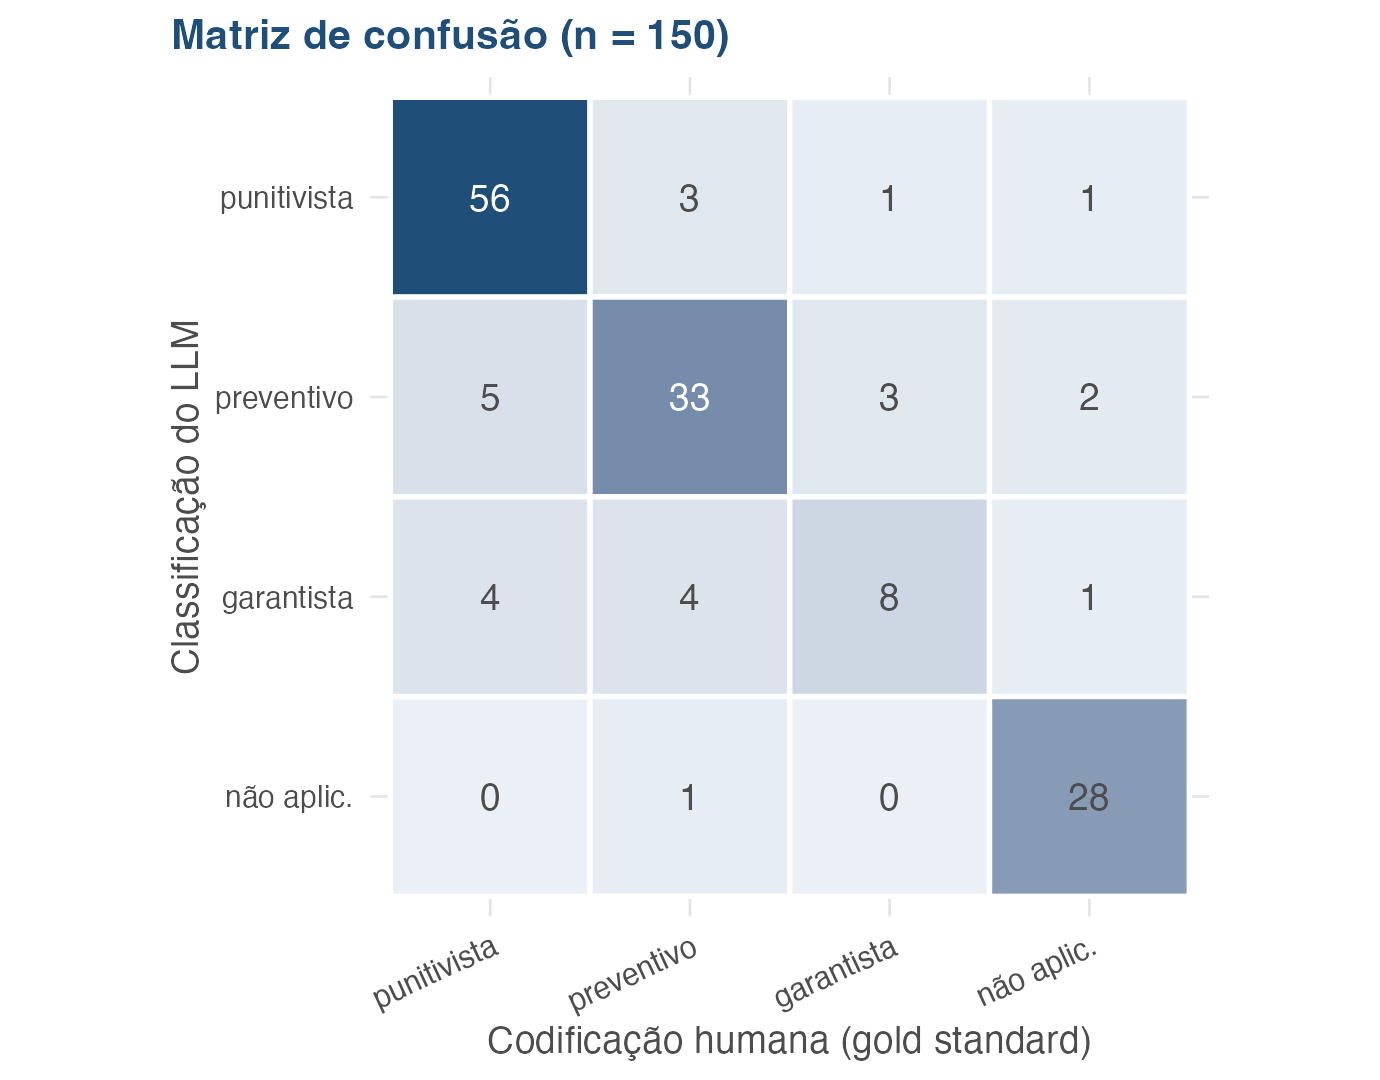
\includegraphics[width=0.94\linewidth]{figuras/fig_confusao.png}
\end{columns}
\end{frame}

% --- SLIDE 10/10 --------------------------------------------------------------
\begin{frame}{O mínimo inegociável, em cinco linhas}
\begin{enumerate}
  \item Rotule uma \textbf{amostra aleatória por humanos}, mesmo pequena, entre
        100 e 300 documentos. Ela é o seu \emph{gold standard}.
  \vspace{0.08cm}
  \item Reporte $\kappa$, $\alpha$ e AC1 \textbf{por categoria}, com a matriz de
        confusão.
  \vspace{0.08cm}
  \item Rode um \emph{baseline} simples antes do modelo complexo, e mostre os
        dois.
  \vspace{0.08cm}
  \item Trate rótulos de máquina como \textbf{medida com erro}, e não como dado
        observado.
  \vspace{0.08cm}
  \item Deposite \emph{prompt}, versão do modelo, \emph{outputs} brutos e
        \texttt{sessionInfo()} em repositório público.
\end{enumerate}
\vspace{0.25cm}
\centering
\small O detalhamento de cada item está no apêndice, ao final deste arquivo.
\end{frame}

% =============================================================================
\section{Atividade}
% =============================================================================

% --- ATIVIDADE (13h55 às 14h30) ----------------------------------------------
\begin{frame}{Atividade: 35 minutos, individual, no seu próprio projeto}
\begin{block}{Objetivo}
Sair daqui com o esqueleto validável de uma medida de texto para \textbf{a sua
própria pesquisa}, já submetido a um teste de confiabilidade.
\end{block}
\vspace{0.15cm}
\begin{table}
\scriptsize
\begin{tabular}{p{1.3cm}p{5.4cm}p{6.1cm}}
\toprule
\textbf{Tempo} & \textbf{Etapa} & \textbf{Produto} \\
\midrule
5 min  & Defina a pergunta e a unidade de registro do seu projeto &
Pergunta e unidade de registro definidas \\
15 min & Escrever o codebook, de 2 a 4 categorias &
Definição, inclusão, exclusão e 2 exemplos-limite por categoria \\
10 min & \textbf{Dupla-codificação interna}: aplique o codebook duas vezes &
5 documentos do seu corpus, codificados em duas rodadas cegas entre si \\
5 min  & Calcular concordância e diagnosticar &
A categoria com maior desacordo, e a reescrita proposta \\
\bottomrule
\end{tabular}
\end{table}
\footnotesize Materiais: \texttt{scripts/06\_atividade.R} (script-modelo do
\texttt{acR}) e \texttt{data/corpus\_atividade.csv} (exemplo, se ainda não
tiver corpus próprio). Quem preferir papel, use papel: o produto é o
raciocínio, não o arquivo.
\end{frame}

\begin{frame}{Como conduzir a dupla-codificação interna}
\begin{columns}[T]
\column{0.49\textwidth}
\textbf{Regras}
\begin{enumerate}\small
  \item Escolha 5 documentos do seu corpus (de preferência, casos difíceis) e
        codifique-os com o codebook: rodada 1.
  \item Depois de alguns minutos, sem consultar a rodada 1, codifique os
        mesmos 5 documentos de novo: rodada 2.
  \item Só então compare as duas rodadas.
\end{enumerate}
\column{0.49\textwidth}
\textbf{O cálculo, sem software}
\vspace{0.1cm}

\small Concordância bruta $=$ acordos entre as duas rodadas dividido por 5.
\vspace{0.15cm}

Com 5 documentos, nenhuma métrica corrigida pelo acaso é confiável. O objetivo
aqui não é o número, é \textbf{localizar o desacordo}.
\end{columns}
\vspace{0.25cm}
\begin{alertblock}{A pergunta que interessa}
\small
Para cada discordância: você leu o documento de forma diferente na segunda
rodada, ou aplicou uma regra diferente? O primeiro caso é problema de
\textbf{unidade de registro}. O segundo, de \textbf{definição}.
\end{alertblock}
\end{frame}

% --- APRESENTAÇÕES (14h30 às 14h50) ------------------------------------------
\begin{frame}{Apresentações: 3 minutos por pessoa}
\textbf{Roteiro fixo. Cronometrado.}
\vspace{0.25cm}
\begin{enumerate}\small
  \item A pergunta de pesquisa e a unidade de registro escolhida. \hfill (30 s)
  \item Uma categoria do codebook, lida em voz alta. \hfill (30 s)
  \item A categoria com maior desacordo entre as duas rodadas, e o
        diagnóstico: circular, não exaustiva, não exclusiva, abstrata demais
        ou rara demais? \hfill (60 s)
  \item A reescrita proposta para essa definição. \hfill (30 s)
  \item Qual método você usaria, entre dicionário, supervisionado e LLM, e por
        quê. \hfill (30 s)
\end{enumerate}
\vspace{0.25cm}
\begin{block}{Papel da plateia}
\small
Quem apresenta recebe \textbf{uma} pergunta de outro participante, escolhido
pelo facilitador. Pergunta, não sugestão. A melhor costuma ser: ``que
documento faria essa categoria falhar?''
\end{block}
\end{frame}

\begin{frame}{O critério de sucesso desta atividade}
\begin{alertblock}{Não é ter um codebook perfeito}
É ter descoberto onde ele quebra \textbf{antes} de gastar dinheiro, tempo e
reputação.
\end{alertblock}
\vspace{0.4cm}
\centering
\large
Quem apresenta um desacordo bem diagnosticado\\
aprendeu mais do que quem apresenta\\
concordância perfeita em cinco documentos fáceis.
\vspace{0.5cm}

\small Se o seu codebook sobreviveu intacto ao teste, desconfie: ou as
categorias são triviais, ou os cinco documentos eram fáceis demais.
\end{frame}

% --- FECHAMENTO (14h50 às 15h00) ---------------------------------------------
\begin{frame}{As próximas duas semanas, no seu projeto}
\begin{enumerate}\small
  \item \textbf{Semana 1.} Monte o corpus e rode apenas descritivas. Leia 30
        documentos a olho. Você vai revisar o codebook depois disso, e todo
        mundo revisa.
  \vspace{0.12cm}
  \item \textbf{Semana 1.} Codifique 50 documentos manualmente. Meça
        concordância com um colega. Reescreva o codebook.
  \vspace{0.12cm}
  \item \textbf{Semana 2.} Rode o \emph{baseline} de dicionário e o LLM em 300
        documentos. Compare com os seus 50 rótulos humanos.
  \vspace{0.12cm}
  \item \textbf{Semana 2.} Só então escale. E deposite tudo em repositório
        público desde o primeiro dia, não no fim.
\end{enumerate}
\vspace{0.2cm}
\begin{block}{Fico à disposição}
\footnotesize
Dúvidas sobre o \texttt{acR}, \emph{issues} e sugestões:
\texttt{github.com/andersonheri/acR/issues} $\bullet$ andersonheri@gmail.com
\end{block}
\end{frame}

\begin{frame}{Síntese das duas aulas}
\begin{enumerate}
  \item A escala não relaxa nenhuma exigência metodológica. Ela transfere o ônus
        da codificação para a auditoria.
  \item Identifique a tarefa antes da ferramenta, e use \emph{baseline} sempre.
  \item Pré-processamento é decisão teórica e precisa ser reportado.
  \item Concordância se reporta por categoria, com mais de uma métrica e com a
        matriz de confusão.
  \item Rótulos gerados por máquina carregam erro sistemático.
  \item Transparência é o que separa análise automatizada de texto de geração
        automatizada de números.
\end{enumerate}
\vspace{0.2cm}
\centering
\small \textit{``Validate, validate, validate''}, Grimmer e Stewart (2013).
Treze anos depois, com LLMs, o conselho ficou mais urgente.
\end{frame}

% =============================================================================
\section*{Referências}
% =============================================================================

\begin{frame}{Referências (1 de 2)}
\scriptsize
\begin{block}{Base metodológica}
GRIMMER, Justin; ROBERTS, Margaret E.; STEWART, Brandon M. \textbf{Text as Data:
a new framework for machine learning and the social sciences}. Princeton:
Princeton University Press, 2022.\\[2pt]
BARBERÁ, Pablo et al. Automated text classification of news articles: a
practical guide. \textit{Political Analysis}, v. 29, n. 1, p. 19--42, 2021.\\[2pt]
KRIPPENDORFF, Klaus. \textbf{Content Analysis: an introduction to its
methodology}. 4. ed. Thousand Oaks: Sage, 2018.\\[2pt]
SAMPAIO, Rafael Cardoso; LYCARIÃO, Diógenes. \textbf{Análise de conteúdo
categorial: manual de aplicação}. Brasília: Enap, 2021.
\end{block}
\end{frame}

\begin{frame}{Referências (2 de 2)}
\scriptsize
\begin{block}{LLMs, confiabilidade e software}
GILARDI, Fabrizio; ALIZADEH, Meysam; KUBLI, Maël. ChatGPT outperforms crowd
workers for text-annotation tasks. \textit{PNAS}, v. 120, n. 30, 2023.\\[2pt]
WANG, Xuezhi et al. Self-consistency improves chain of thought reasoning in
language models. \textit{EMNLP}, 2023.\\[2pt]
GWET, Kilem L. \textbf{Handbook of Inter-Rater Reliability}. 4. ed.
Gaithersburg: Advanced Analytics, 2014.\\[2pt]
BENOIT, Kenneth et al. quanteda: an R package for the quantitative analysis of
textual data. \textit{Journal of Open Source Software}, v. 3, n. 30, 2018.\\[2pt]
HENRIQUE, Anderson. \textbf{acR}: análise de conteúdo em R. Pacote R versão
0.3.2, 2026. \texttt{ahenriquecp.com/acR}\\[2pt]
\textit{[VERIFICAR]} Literatura sobre inferência com rótulos imperfeitos,
publicada entre 2023 e 2026.
\end{block}
\end{frame}

% --- ENCERRAMENTO -------------------------------------------------------------
\begin{frame}[plain]
\centering
\vspace{1.0cm}
{\Large \textbf{Obrigado!}}\\[0.45cm]
{\large Anderson Henrique}\\[0.18cm]
\textit{CEM/USP $\bullet$ INCT QualiGov $\bullet$ IPEA}\\[0.18cm]
andersonheri@gmail.com\\[0.7cm]

\small
Materiais, dados e scripts comentados:\\
\texttt{github.com/andersonheri/sicss-brazil-2026-text}\\[0.12cm]
Pacote \texttt{acR}: \texttt{ahenriquecp.com/acR}\\[0.7cm]

\parbox{0.85\textwidth}{\scriptsize
\textbf{Como citar:} HENRIQUE, Anderson. \textit{Análise Automatizada de Texto:
oficina de codebook, validação e reprodutibilidade em R}. 2026. Apresentação em
slides: material didático não publicado, elaborado para o Summer Institute in
Computational Social Science, Brazil (SICSS-Brazil 2026), Fundação Getulio
Vargas, Rio de Janeiro. CEM-USP / INCT QualiGov.}

\end{frame}

% =============================================================================
%  APÊNDICE
%  Conteúdo retirado da exposição para liberar tempo de oficina.
%  Use sob demanda, durante a atividade ou nas perguntas.
% =============================================================================

\appendix

\begin{frame}[plain]
\centering
\vspace{1.6cm}
{\Huge \textbf{Apêndice}}\\[0.7cm]
{\large Material de consulta}\\[0.5cm]
\small
\parbox{0.75\textwidth}{\centering
Estes slides não fazem parte da exposição de 20 minutos. Estão aqui para as
dúvidas da oficina e para consulta posterior.}
\end{frame}

% --- A1 -----------------------------------------------------------------------
\begin{frame}{A1. Três estratégias de classificação}
\begin{table}
\scriptsize
\begin{tabular}{p{2.3cm}p{3.1cm}p{3.2cm}p{3.4cm}}
\toprule
& \textbf{Dicionário} & \textbf{Supervisionado} & \textbf{LLM zero/few-shot} \\
\midrule
Custo inicial & Baixo, construir a lista & Alto, rotular de 500 a 2.000 docs &
Baixo, escrever o codebook \\
\addlinespace
Custo marginal & Zero & Zero após treinar & Por documento, via API \\
\addlinespace
Transparência & Total & Média, pesos inspecionáveis & Baixa \\
\addlinespace
Reprodutibilidade & Total & Total, com \emph{seed} & Parcial, depende da versão \\
\addlinespace
Capta o latente & Não & Pouco & Sim, em parte \\
\addlinespace
Falha quando & O vocabulário muda; há ironia & O domínio muda &
A categoria é idiossincrática do seu campo \\
\bottomrule
\end{tabular}
\end{table}
\vspace{0.1cm}
\footnotesize \textbf{Recomendação:} comece pelo dicionário como \emph{baseline}.
Se ele resolve, você economizou dinheiro e ganhou transparência.
\end{frame}

% --- A2 -----------------------------------------------------------------------
\begin{frame}{A2. A escada de \emph{baselines}}
\begin{block}{Um resultado que a literatura repete}
Modelos complexos costumam superar modelos simples por margens pequenas em
classificação de texto político. Sem \emph{baseline}, você não sabe se o ganho
justificou o custo, a opacidade e a perda de replicabilidade.
\end{block}
\vspace{0.25cm}
\begin{enumerate}\small
  \item Classe majoritária, que é o piso absoluto.
  \item Dicionário construído a partir do seu codebook.
  \item Regressão logística ou Naive Bayes sobre a matriz documento-termo.
  \item LLM \emph{zero-shot}.
  \item LLM \emph{few-shot} com exemplos do seu corpus.
\end{enumerate}
\vspace{0.15cm}
\footnotesize \textbf{Reporte todos.} Uma tabela com cinco linhas e a coluna
$F_1$ por classe é uma das seções de métodos mais convincentes que você pode
escrever.
\end{frame}

% --- A3 -----------------------------------------------------------------------
\begin{frame}[fragile]{A3. Código do \emph{baseline} supervisionado}
\begin{lstlisting}
library(quanteda); library(quanteda.textmodels)
set.seed(1234)

# Particao ESTRATIFICADA pela classe (importante com classes raras)
idx <- caret::createDataPartition(rotulos$categoria, p = .8, list = FALSE)

mod_nb <- textmodel_nb(dfm_treino[idx, ], rotulos$categoria[idx])
pred   <- predict(mod_nb, newdata = dfm_teste)

caret::confusionMatrix(pred, rotulos$categoria[-idx], mode = "prec_recall")
\end{lstlisting}
\begin{lstlisting}[style=Rsaida]
Accuracy : 0.7533   (No Information Rate : 0.4067)
                    Precision  Recall    F1
Class: punitivista     0.8033   0.8033  0.8033
Class: preventivo      0.7000   0.6512  0.6747
Class: garantista      0.4444   0.2353  0.3077   <- classe rara falha
Class: nao_aplicavel   0.8710   0.9310  0.9000
\end{lstlisting}
\end{frame}

% --- A4 -----------------------------------------------------------------------
\begin{frame}{A4. Três armadilhas no código anterior}
\begin{enumerate}
  \item \textbf{Partição não estratificada.}\\
        \small Com classes raras, uma partição aleatória simples pode deixar a
        categoria ``garantista'' quase ausente do treino.
  \vspace{0.2cm}
  \item \normalsize \textbf{Vazamento de informação.}\\
        \small Construir a matriz documento-termo antes de separar treino e
        teste faz o vocabulário do teste influenciar o treino.
  \vspace{0.2cm}
  \item \normalsize \textbf{Acurácia global como métrica.}\\
        \small Se 70\% do corpus é uma só classe, um classificador trivial
        atinge 70\% de acurácia sem aprender nada. Compare sempre com a taxa de
        não informação.
\end{enumerate}
\end{frame}

% --- A5 -----------------------------------------------------------------------
\begin{frame}{A5. Categorias definidas por você ou pelo modelo?}
\begin{columns}[T]
\column{0.48\textwidth}
\textbf{Categorias \emph{a priori}}
\begin{itemize}\small
  \item Você define a partir da teoria.
  \item Corresponde à análise de conteúdo dedutiva.
  \item Recomendado quando há literatura consolidada.
\end{itemize}
\column{0.48\textwidth}
\textbf{Categorias emergentes}
\begin{itemize}\small
  \item Úteis na fase exploratória.
  \item Mas, se o modelo propõe as categorias e também as aplica, não há
        validação independente.
\end{itemize}
\end{columns}
\vspace{0.3cm}
\begin{alertblock}{O problema epistemológico}
\small
Deixar o LLM inferir as categorias e depois usá-lo para codificar cria
circularidade: a concordância medida é a consistência interna do modelo, não a
validade da categoria. Nesse caso, a validação humana passa a ser obrigatória.
\end{alertblock}
\end{frame}

% --- A6 -----------------------------------------------------------------------
\begin{frame}{A6. Amostrar por incerteza ou aleatoriamente?}
\begin{columns}[T]
\column{0.48\textwidth}
\textbf{Por incerteza}
\begin{itemize}\small
  \item Concentra o esforço humano onde o modelo hesitou.
  \item Diagnostica o codebook com eficiência.
  \item \textbf{Superestima} o desacordo.
\end{itemize}
\column{0.48\textwidth}
\textbf{Aleatória}
\begin{itemize}\small
  \item Estima a acurácia populacional sem viés.
  \item Permite corrigir estimativas a jusante.
  \item Desperdiça esforço nos casos fáceis.
\end{itemize}
\end{columns}
\vspace{0.35cm}
\begin{block}{Faça as duas, e reporte separadamente}
\small
A amostra aleatória é o seu \emph{gold standard} para inferência. A amostra por
incerteza é a sua ferramenta de diagnóstico. Confundir as duas produz uma taxa
de erro que não descreve nem uma coisa nem outra.
\end{block}
\end{frame}

% --- A7 -----------------------------------------------------------------------
\begin{frame}{A7. Erro de medida: rótulos de máquina não são dados}
\begin{block}{O problema}
Se você usa $\hat{Y}$, o rótulo do modelo, como se fosse $Y$, a categoria
verdadeira, em uma regressão, os coeficientes ficam enviesados. E o viés não
desaparece com $N$ maior, porque os erros de classificação são sistemáticos.
\end{block}
\vspace{0.3cm}
\centering
\begin{tikzpicture}[node distance=0.5cm]
  \node[alerta, minimum width=4.8cm] (a) {Ingênuo\\$\hat{Y}$ tratado como $Y$\\
        gera viés de atenuação ou inflação};
  \node[destaque, minimum width=4.8cm, right=0.9cm of a] (b) {Correto\\
        amostra humana pequena\\somada à amostra grande\\gera estimador corrigido};
  \draw[seta] (a) -- (b);
\end{tikzpicture}
\vspace{0.3cm}

\small \textbf{Intuição da correção:} use a amostra rotulada por humanos para
estimar a taxa de erro do classificador e ajustar a estimativa obtida na amostra
grande. É o mesmo raciocínio de calibração usado com dados administrativos
imperfeitos.
\end{frame}

% --- A8 -----------------------------------------------------------------------
\begin{frame}{A8. Riscos que exigem tratamento explícito no artigo}
\begin{enumerate}\small
  \item \textbf{Não determinismo.} O mesmo \emph{prompt}, em datas diferentes,
        pode gerar rótulos diferentes. Fixe versão, temperatura e \emph{seed},
        e reporte a data de execução.
  \vspace{0.1cm}
  \item \textbf{Opacidade e contaminação.} Você não sabe o que há no treino.
        Contaminação com o próprio corpus é possível e indetectável.
  \vspace{0.1cm}
  \item \textbf{Viés de posição e de rótulo.} Modelos favorecem categorias
        listadas primeiro. Teste embaralhando a ordem.
  \vspace{0.1cm}
  \item \textbf{Deriva de versão.} O provedor atualiza o modelo e seu resultado
        deixa de replicar. Salve os \emph{outputs} brutos.
  \vspace{0.1cm}
  \item \textbf{Custo financeiro e energético.} Reporte o volume de chamadas.
\end{enumerate}
\vspace{0.2cm}
\begin{block}{Regra que proponho}
\footnotesize O \emph{output} bruto do modelo é \textbf{dado primário} e deve ser
depositado junto com o corpus. Sem isso, o trabalho é irreplicável por
construção.
\end{block}
\end{frame}

% --- A9 -----------------------------------------------------------------------
\begin{frame}[fragile]{A9. Relatório reprodutível}
\begin{lstlisting}
# Relatorio metodologico automatico: codebook, parametros,
# metricas, amostra auditada e sessionInfo
ac_qual_report(resultado, codebook = codebook, reliability = confiab,
               format = "html", path = "outputs/relatorio_metodologico.html")

ac_export(resultado, path = "outputs/classificacao.csv")
ac_export(irr,       path = "outputs/metricas.tex")   # direto para o artigo

writeLines(capture.output(sessionInfo()), "outputs/sessionInfo.txt")
\end{lstlisting}
\vspace{0.2cm}
\begin{block}{O que vai para o repositório público}
\small
Corpus, quando a licença permitir; codebook; \emph{prompts} completos;
\emph{outputs} brutos do modelo; planilha de codificação humana anonimizada;
scripts numerados; \texttt{sessionInfo()}; e \texttt{renv.lock}.
\end{block}
\end{frame}

% --- A10 ----------------------------------------------------------------------
\begin{frame}{A10. \emph{Checklist} de reporte}
\begin{columns}[T]
\column{0.49\textwidth}
\textbf{Desenho}
\begin{itemize}\scriptsize
  \item[$\square$] Unidade de amostragem, registro e contexto
  \item[$\square$] Critério de inclusão no corpus e período
  \item[$\square$] Codebook completo em anexo
  \item[$\square$] Todas as decisões de pré-processamento
\end{itemize}
\vspace{0.15cm}
\textbf{Classificação}
\begin{itemize}\scriptsize
  \item[$\square$] \emph{Baseline} e comparação
  \item[$\square$] Modelo, versão exata e data de execução
  \item[$\square$] \emph{Prompt} completo, não parafraseado
  \item[$\square$] Parâmetros: temperatura, $k$ e \emph{seed}
\end{itemize}
\column{0.49\textwidth}
\textbf{Validação}
\begin{itemize}\scriptsize
  \item[$\square$] $n$ e estratégia da amostra humana
  \item[$\square$] Número de codificadores e treinamento
  \item[$\square$] $\kappa$, $\alpha$ e AC1 por categoria
  \item[$\square$] Matriz de confusão
  \item[$\square$] $F_1$ por classe
\end{itemize}
\vspace{0.15cm}
\textbf{Transparência}
\begin{itemize}\scriptsize
  \item[$\square$] Repositório público
  \item[$\square$] \texttt{sessionInfo()} e \texttt{renv.lock}
  \item[$\square$] Declaração de uso de IA
  \item[$\square$] Limitações por categoria
\end{itemize}
\end{columns}
\end{frame}

\end{document}
